% !TeX program = xelatex
\documentclass[a4paper,10pt]{article}

% ============================================================================
% ១. កញ្ចប់បណ្ណាល័យ និងការកំណត់ទំព័រ (Packages & Page Setup — តាមគំរូ ls_plan.tex)
% ============================================================================
\usepackage[a4paper, left=0.95cm, right=0.95cm, top=0.85cm, bottom=0.92cm, footskip=0.52cm]{geometry}
\usepackage{amsmath}
\usepackage{unicode-math}
\usepackage{fontspec}
\usepackage{longtable, array, multirow, colortbl}
\usepackage[table]{xcolor}
\usepackage{enumitem}
\usepackage{pifont}
\usepackage{fancyhdr}
\usepackage{tikz}
\usetikzlibrary{calc, arrows.meta, decorations.pathreplacing, patterns, positioning, babel}

\makeatletter
\let\@expl@@@mark@update@singlecol@structures@@\relax
\makeatother

% --- ប្រព័ន្ធស្វែងរកទីតាំងពុម្ពអក្សរស្វ័យប្រវត្តិ (Windows Local + Cloud Repo fonts/) ---
\providecommand{\NGSFindFonts}{%
  \IfFileExists{C:/Windows/Fonts/cambria.ttc}{%
    \def\NGSSysPath{C:/Windows/Fonts/}%
    \def\NGSUserPath{C:/Users/KIT/AppData/Local/Microsoft/Windows/Fonts/}%
  }{%
    \IfFileExists{./fonts/KhmerOSsiemreap.ttf}{\def\NGSSysPath{./fonts/}\def\NGSUserPath{./fonts/}}{%
    \IfFileExists{../fonts/KhmerOSsiemreap.ttf}{\def\NGSSysPath{../fonts/}\def\NGSUserPath{../fonts/}}{%
    \IfFileExists{../../fonts/KhmerOSsiemreap.ttf}{\def\NGSSysPath{../../fonts/}\def\NGSUserPath{../../fonts/}}{%
    \IfFileExists{../../../fonts/KhmerOSsiemreap.ttf}{\def\NGSSysPath{../../../fonts/}\def\NGSUserPath{../../../fonts/}}{%
    \IfFileExists{../../../../fonts/KhmerOSsiemreap.ttf}{\def\NGSSysPath{../../../../fonts/}\def\NGSUserPath{../../../../fonts/}}{%
    \IfFileExists{../../../../../fonts/KhmerOSsiemreap.ttf}{\def\NGSSysPath{../../../../../fonts/}\def\NGSUserPath{../../../../../fonts/}}{%
    \IfFileExists{../../../../../../fonts/KhmerOSsiemreap.ttf}{\def\NGSSysPath{../../../../../../fonts/}\def\NGSUserPath{../../../../../../fonts/}}{%
      \def\NGSSysPath{../../../../../../../fonts/}\def\NGSUserPath{../../../../../../../fonts/}%
    }}}}}}}%
  }%
}
\NGSFindFonts

% ============================================================================
% ២. កំណត់ពុម្ពអក្សរ (Fonts — តាមគំរូ ls_plan.tex)
% ============================================================================
\setmathfont[Path={\NGSSysPath}, FontIndex=1, Scale=1.02]{cambria.ttc}
\defaultfontfeatures{Ligatures=TeX}

\setmainfont[
  Path={\NGSUserPath},
  Extension=.ttf,
  Script=Khmer,
  BoldFont={KhmerOSsiemreap},
  BoldFeatures={FakeBold=1.8},
  ItalicFont={KhmerOSsiemreap},
  ItalicFeatures={FakeSlant=0.25},
  BoldItalicFont={KhmerOSsiemreap},
  BoldItalicFeatures={FakeBold=1.8, FakeSlant=0.25}
]{KhmerOSsiemreap}

\newfontfamily\muol[Path={\NGSUserPath}, Extension=.ttf, Script=Khmer]{KhmerOSmuollight}
\newfontfamily\Tacteing[Path={\NGSUserPath}, Extension=.TTF]{TACTENG}
\newfontfamily\TimesEn[Path={\NGSSysPath}, Extension=.ttf, BoldFont={timesbd}, ItalicFont={timesi}, BoldItalicFont={timesbi}]{times}
\newfontfamily\CalibriFont[Path={\NGSSysPath}, Extension=.ttf]{calibri}
\newfontfamily\CourierCirc[Path={\NGSSysPath}, Extension=.ttf]{cour}

\XeTeXlinebreaklocale "km"
\XeTeXlinebreakskip = 0pt plus 1pt minus 0.1pt

% ============================================================================
% ៣. ពណ៌ និងការតុបតែង (Colors & Styles)
% ============================================================================
\definecolor{stepbg}{HTML}{D9D9D9}
\definecolor{headgray}{HTML}{E6E6E6}
\definecolor{emphred}{HTML}{C00000}

\pagestyle{fancy}
\fancyhf{}
\renewcommand{\headrulewidth}{0pt}
\fancyfoot[R]{\CalibriFont\fontsize{9pt}{11pt}\selectfont\thepage}

\setlength{\parindent}{0pt}
\setlength{\parskip}{0pt}
\setlength{\tabcolsep}{4.5pt}
\setlength{\LTpre}{2pt}
\setlength{\LTpost}{2pt}

\newcolumntype{L}[1]{>{\raggedright\arraybackslash}p{#1}}
\newcolumntype{C}[1]{>{\centering\arraybackslash}p{#1}}

% ============================================================================
% ៤. ពាក្យបញ្ជាជំនួយ (Helper Macros)
% ============================================================================
\newcommand{\en}[1]{{\TimesEn #1}}
\newcommand{\enbf}[1]{{\TimesEn\bfseries #1}}
\newcommand{\khmflourish}{{\Tacteing\fontsize{15pt}{15pt}\selectfont 3}}
\newcommand{\wcirc}{{\CourierCirc\fontsize{9.5pt}{11pt}\selectfont o}}
\newcommand{\ditem}{{\fontsize{7.5pt}{10pt}\selectfont\ding{117}}\ }
\newcommand{\fiveE}[1]{\textcolor{emphred}{\CalibriFont\bfseries #1}}
\newcommand{\redsub}[1]{\textcolor{emphred}{#1}}
\newcommand{\timenote}[1]{\textcolor{emphred}{\textit{#1}}}
\newcommand{\stepheader}[1]{\multicolumn{3}{|c|}{\cellcolor{stepbg}\muol #1} \\ \hline}
\newcommand{\cfig}[1]{{\centering\vspace{3pt}#1\vspace{3pt}\par}}
\newcommand{\cnum}[1]{\mbox{\fontsize{10.5pt}{12pt}\selectfont\ding{\numexpr181+#1\relax}}}
\newcommand{\unit}[1]{\,\text{\en{#1}}}
\newcommand{\riel}{\,\text{៛}}
\newcommand{\graybox}[1]{\colorbox{headgray}{\strut #1}}

% ============================================================================
% ៥. រូបភាព TikZ ស-ខ្មៅ សម្រាប់បង្រៀនលើក្ដារខៀន និងសន្លឹកកិច្ចការ (B&W Diagrams)
% ============================================================================

% ១. E1 Engage: បេសកកម្មអន្ទាក់ម៉ោងនិងនាទីលើម៉ូតូរត់បាន 108 km ក្នុង 2h 15mn
\newcommand{\figEngageMEASFourFour}{%
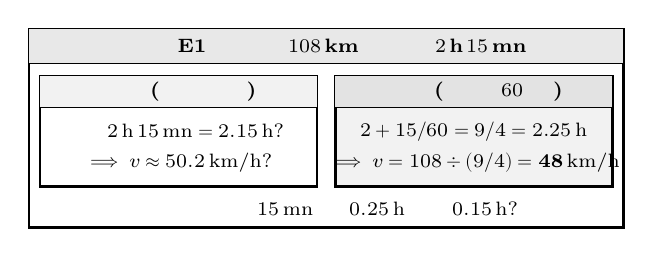
\begin{tikzpicture}[x=1cm, y=1cm, every node/.style={font=\scriptsize, text=black}]
  \draw[black, line width=0.9pt] (0,0) rectangle (7.55,2.52);
  \fill[gray!18] (0,2.08) rectangle (7.55,2.52);
  \draw[black, line width=0.6pt] (0,2.08) -- (7.55,2.08);
  \node at (3.775,2.30) {\textbf{បេសកកម្ម \en{E1}៖ ម៉ូតូរត់បាន $108\unit{km}$ ក្នុងរយៈពេល $2\unit{h}\,15\unit{mn}$}};

  % Left: Student A (Decimal base-10 trap)
  \draw[black, line width=0.8pt] (0.14,0.52) rectangle (3.66,1.92);
  \fill[gray!10] (0.14,1.52) rectangle (3.66,1.92);
  \draw[black, line width=0.5pt] (0.14,1.52) -- (3.66,1.52);
  \node at (1.90,1.72) {\textbf{សិស្ស ក (គិតជាទសភាគផ្ទាល់)}};
  \node at (1.90,1.22) {ប្ដូរ $2\unit{h}\,15\unit{mn} = 2.15\unit{h}$?};
  \node at (1.90,0.82) {$\implies v \approx 50.2\unit{km/h}$?};

  % Right: Student B (Base-60 truth)
  \draw[black, line width=0.95pt, fill=gray!10] (3.89,0.52) rectangle (7.41,1.92);
  \fill[gray!22] (3.89,1.52) rectangle (7.41,1.92);
  \draw[black, line width=0.55pt] (3.89,1.52) -- (7.41,1.52);
  \node at (5.65,1.72) {\textbf{សិស្ស ខ (គិតតាមគោល $60$ នាទី)}};
  \node at (5.65,1.22) {$2 + 15/60 = 9/4 = 2.25\unit{h}$};
  \node at (5.65,0.82) {$\implies v = 108 \div (9/4) = \mathbf{48\unit{km/h}}$};

  \node at (3.775,0.24) {\textbf{សំណួរគន្លឹះ៖} ហេតុអ្វី $15\unit{mn}$ ស្មើ $0.25\unit{h}$ មិនមែន $0.15\unit{h}$?};
\end{tikzpicture}}

% ២. E2 Explore: បន្ទាត់ចំនួនពីរជួរនៃឧទាហរណ៍ទី ១ (ទំ.៤៩ — 108 km ក្នុង 9/4 h)
\newcommand{\figMotoSpeedMEASFourFour}{%
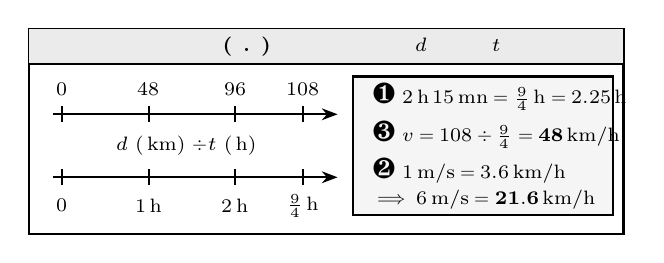
\begin{tikzpicture}[x=1cm, y=1cm, every node/.style={font=\scriptsize, text=black}]
  \draw[black, line width=0.9pt] (0,0) rectangle (7.55,2.60);
  \fill[gray!16] (0,2.16) rectangle (7.55,2.60);
  \draw[black, line width=0.6pt] (0,2.16) -- (7.55,2.16);
  \node at (3.775,2.38) {\textbf{ឧទាហរណ៍ទី ១ (ទំ.៤៩)៖ បន្ទាត់ពីរជួរ ចម្ងាយចរ $d$ និងរយៈពេល $t$}};

  % Double number line on left
  \draw[-{Stealth[length=2mm]}, black, line width=0.85pt] (0.30,1.52) -- (3.92,1.52);
  \draw[-{Stealth[length=2mm]}, black, line width=0.85pt] (0.30,0.72) -- (3.92,0.72);
  \foreach \x/\d/\t in {0.42/0/0, 1.52/48/1\unit{h}, 2.62/96/2\unit{h}, 3.48/108/\tfrac{9}{4}\unit{h}} {
    \draw[black, line width=0.75pt] (\x,1.42) -- (\x,1.62);
    \draw[black, line width=0.75pt] (\x,0.62) -- (\x,0.82);
    \node at (\x,1.84) {$\d$};
    \node at (\x,0.36) {$\t$};
  }
  \node at (2.00,1.12) {$d$ ($\unit{km}$) $\div t$ ($\unit{h}$)};

  % Calculation box on right
  \draw[black, line width=0.8pt, fill=gray!8] (4.12,0.24) rectangle (7.42,2.00);
  \node[anchor=west] at (4.24,1.74) {\cnum{1} $2\unit{h}\,15\unit{mn} = \tfrac{9}{4}\unit{h} = 2.25\unit{h}$};
  \node[anchor=west] at (4.24,1.26) {\cnum{3} $v = 108\div \tfrac{9}{4} = \mathbf{48\unit{km/h}}$};
  \node[anchor=west] at (4.24,0.80) {\cnum{2} $1\unit{m/s} = 3.6\unit{km/h}$};
  \node[anchor=west] at (4.24,0.44) {$\implies 6\unit{m/s} = \mathbf{21.6\unit{km/h}}$};
\end{tikzpicture}}

% ៣. E3 Explain: ស្ពានបំប្លែងខ្នាត m/s <-> km/h និងត្រីកោណរូបមន្ត v = d/t
\newcommand{\figSpeedBridgeMEASFourFour}{%
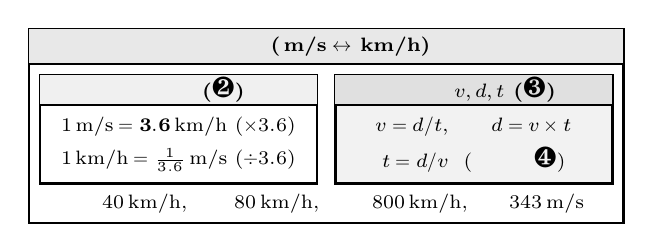
\begin{tikzpicture}[x=1cm, y=1cm, every node/.style={font=\scriptsize, text=black}]
  \draw[black, line width=0.9pt] (0,0) rectangle (7.55,2.46);
  \fill[gray!18] (0,2.02) rectangle (7.55,2.46);
  \draw[black, line width=0.6pt] (0,2.02) -- (7.55,2.02);
  \node at (3.775,2.24) {\textbf{ស្ពានបំប្លែងខ្នាតល្បឿន ($\unit{m/s} \leftrightarrow \unit{km/h}$) និងរូបមន្តគោល}};

  % Left box: Speed unit bridge
  \draw[black, line width=0.8pt] (0.14,0.50) rectangle (3.66,1.88);
  \fill[gray!12] (0.14,1.50) rectangle (3.66,1.88);
  \draw[black, line width=0.55pt] (0.14,1.50) -- (3.66,1.50);
  \node at (1.90,1.69) {\textbf{ស្ពានខ្នាតល្បឿន (\cnum{2})}};
  \node at (1.90,1.22) {$1\unit{m/s} = \mathbf{3.6\unit{km/h}}$ ($\times 3.6$)};
  \node at (1.90,0.80) {$1\unit{km/h} = \tfrac{1}{3.6}\unit{m/s}$ ($\div 3.6$)};

  % Right box: Formula relations
  \draw[black, line width=0.95pt, fill=gray!10] (3.89,0.50) rectangle (7.41,1.88);
  \fill[gray!24] (3.89,1.50) rectangle (7.41,1.88);
  \draw[black, line width=0.6pt] (3.89,1.50) -- (7.41,1.50);
  \node at (5.65,1.69) {\textbf{ទំនាក់ទំនង $v, d, t$ (\cnum{3})}};
  \node at (5.65,1.22) {$v = d / t, \qquad d = v \times t$};
  \node at (5.65,0.80) {$t = d / v$ \ (ឯកភាពខ្នាត \cnum{4})};

  \node at (3.775,0.24) {ម៉ូតូ $40\unit{km/h}$, រថយន្ត $80\unit{km/h}$, យន្តហោះ $800\unit{km/h}$, សំឡេង $343\unit{m/s}$};
\end{tikzpicture}}

% ៤. E4 Elaborate: លំហាត់គំរូកាំភ្លើងធំពីទីក្រុង A ទៅទីក្រុង B (ទំ.៤៩)
\newcommand{\figSoundDistanceMEASFourFour}{%
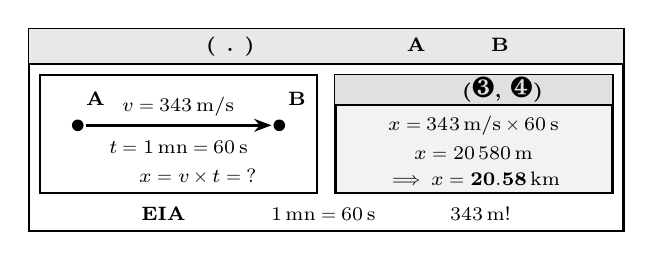
\begin{tikzpicture}[x=1cm, y=1cm, every node/.style={font=\scriptsize, text=black}]
  \draw[black, line width=0.9pt] (0,0) rectangle (7.55,2.56);
  \fill[gray!18] (0,2.12) rectangle (7.55,2.56);
  \draw[black, line width=0.6pt] (0,2.12) -- (7.55,2.12);
  \node at (3.775,2.34) {\textbf{លំហាត់គំរូ (ទំ.៤៩)៖ សំឡេងកាំភ្លើងធំពីទីក្រុង \en{A} ទៅទីក្រុង \en{B}}};

  % Left schematic A -> B
  \draw[black, line width=0.8pt] (0.14,0.48) rectangle (3.66,1.98);
  \fill[black] (0.62,1.34) circle (2.1pt);
  \fill[black] (3.18,1.34) circle (2.1pt);
  \draw[-{Stealth[length=2.2mm]}, black, line width=0.9pt] (0.72,1.34) -- (3.08,1.34);
  \node at (0.62,1.68) {\textbf{ក្រុង \en{A}}};
  \node at (3.18,1.68) {\textbf{ក្រុង \en{B}}};
  \node at (1.90,1.58) {$v = 343\unit{m/s}$};
  \node at (1.90,1.06) {$t = 1\unit{mn} = 60\unit{s}$};
  \node at (1.90,0.70) {ចម្ងាយ $x = v \times t = ?$};

  % Right calculation box
  \draw[black, line width=0.95pt, fill=gray!10] (3.89,0.48) rectangle (7.41,1.98);
  \fill[gray!24] (3.89,1.60) rectangle (7.41,1.98);
  \draw[black, line width=0.6pt] (3.89,1.60) -- (7.41,1.60);
  \node at (5.65,1.79) {\textbf{ជំហានគណនា (\cnum{3}, \cnum{4})}};
  \node at (5.65,1.34) {$x = 343\unit{m/s}\times 60\unit{s}$};
  \node at (5.65,0.98) {$x = 20\,580\unit{m}$};
  \node at (5.65,0.66) {$\implies x = \mathbf{20.58\unit{km}}$};

  \node at (3.775,0.22) {\textbf{\en{EIA}៖} បើភ្លេចប្ដូរ $1\unit{mn} = 60\unit{s}$ នឹងខុសឃើញតែ $343\unit{m}$!};
\end{tikzpicture}}

% ៥. E5 Evaluate: ជម្រើសវិនិច្ឆ័យ A-D (រថយន្តរត់បាន 90 km ក្នុងរយៈពេល 1h 30mn)
\newcommand{\figExitMEASFourFour}{%
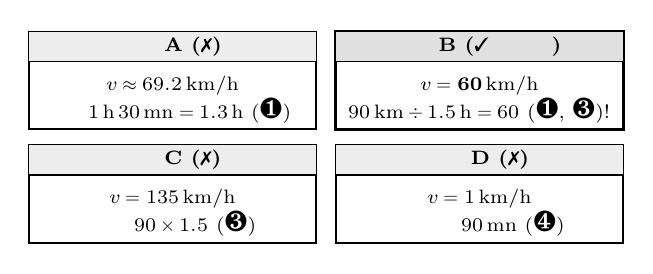
\begin{tikzpicture}[x=1cm, y=1cm, every node/.style={font=\scriptsize, text=black}]
  % Choice A
  \draw[black, line width=0.8pt] (0,1.44) rectangle (3.65,2.68);
  \fill[gray!14] (0,2.30) rectangle (3.65,2.68);
  \draw[black, line width=0.5pt] (0,2.30) -- (3.65,2.30);
  \node at (1.825,2.49) {\textbf{ជម្រើស \en{A} (\ding{55})}};
  \node at (1.825,2.00) {$v \approx 69.2\unit{km/h}$};
  \node at (1.825,1.68) {ច្រឡំ $1\unit{h}\,30\unit{mn} = 1.3\unit{h}$ (\cnum{1})};

  % Choice B (Correct)
  \draw[black, line width=1.05pt] (3.90,1.44) rectangle (7.55,2.68);
  \fill[gray!24] (3.90,2.30) rectangle (7.55,2.68);
  \draw[black, line width=0.6pt] (3.90,2.30) -- (7.55,2.30);
  \node at (5.725,2.49) {\textbf{ជម្រើស \en{B} (\ding{51} ត្រឹមត្រូវ)}};
  \node at (5.725,2.00) {$v = \mathbf{60\unit{km/h}}$};
  \node at (5.725,1.68) {$90\unit{km}\div 1.5\unit{h} = 60$ (\cnum{1}, \cnum{3})!};

  % Choice C
  \draw[black, line width=0.8pt] (0,0) rectangle (3.65,1.24);
  \fill[gray!14] (0,0.86) rectangle (3.65,1.24);
  \draw[black, line width=0.5pt] (0,0.86) -- (3.65,0.86);
  \node at (1.825,1.05) {\textbf{ជម្រើស \en{C} (\ding{55})}};
  \node at (1.825,0.56) {$v = 135\unit{km/h}$};
  \node at (1.825,0.24) {ច្រឡំយក $90\times 1.5$ (\cnum{3})};

  % Choice D
  \draw[black, line width=0.8pt] (3.90,0) rectangle (7.55,1.24);
  \fill[gray!14] (3.90,0.86) rectangle (7.55,1.24);
  \draw[black, line width=0.5pt] (3.90,0.86) -- (7.55,0.86);
  \node at (5.725,1.05) {\textbf{ជម្រើស \en{D} (\ding{55})}};
  \node at (5.725,0.56) {$v = 1\unit{km/h}$};
  \node at (5.725,0.24) {ច្រឡំចែកនឹង $90\unit{mn}$ (\cnum{4})};
\end{tikzpicture}}

\begin{document}
\fontsize{10pt}{15.2pt}\selectfont

% ============================================================================
% ក្បាលរដ្ឋបាល (Administrative Header — តាមគំរូ ls_plan.tex)
% ============================================================================
{\centering
  {\muol\fontsize{11pt}{16pt}\selectfont ព្រះរាជាណាចក្រកម្ពុជា\par}
  {\muol\fontsize{11pt}{16pt}\selectfont ជាតិ សាសនា ព្រះមហាក្សត្រ\par}
  \vspace{-3pt}{\khmflourish\par}
}

\vspace{1pt}
{\muol\fontsize{10pt}{15.5pt}\selectfont
មន្ទីរអប់រំ យុវជន និងកីឡា ខេត្តកំពង់ធំ\par
ការិយាល័យអប់រំ យុវជន និងកីឡា ស្រុកកំពង់ស្វាយ\par
អនុវិទ្យាល័យព្រះក្រសាំង\par}

\vspace{2pt}
{\centering{\muol\fontsize{11.5pt}{17pt}\selectfont កិច្ចតែងការបង្រៀន\par}}
\vspace{2pt}

% --- ព័ត៌មានទូទៅ ---
{\hspace*{2.8cm}\renewcommand{\arraystretch}{1.08}
\begin{tabular}{@{}l@{\hspace{0.35cm}}p{2.9cm}@{\hspace{0.15cm}}c@{\hspace{0.25cm}}l@{}}
  - & មុខវិជ្ជា & : & គណិតវិទ្យា ថ្នាក់ទី៨ (ពីជគណិត) \\
  - & ចំណងជើងមេរៀន & : & មេរៀនទី៤៖ រង្វាស់រង្វាល់ \\
  - & ចំណងជើងរង & : & ៤. ល្បឿនមធ្យម (ទំ.៤៨--៥០) \\
  - & រយៈពេល & : & ១ ម៉ោងសិក្សា (៥០ នាទី) \\
  - & បង្រៀនដោយ & : & ហុក ប៊ុនថែន \\
  - & កាលបរិច្ឆេទ & : & ថ្ងៃព្រហស្បតិ៍ ទី៣ ខែធ្នូ ឆ្នាំ២០២៦ \\
\end{tabular}\par}

\vspace{2pt}

% --- I. វត្ថុបំណង ---
{\muol\fontsize{10pt}{15.5pt}\selectfont \enbf{I.} វត្ថុបំណង\par}
\vspace{1pt}
{\renewcommand{\arraystretch}{1.10}
\begin{tabular}{@{}p{0.55cm}@{}p{2.35cm}@{\hspace{0.15cm}}c@{\hspace{0.25cm}}p{14.95cm}@{}}
  \hfill\wcirc\hspace{0.2cm} & វិជ្ជាសម្បទា & : & សិស្សប្រាប់និយមន័យនិងរូបមន្តល្បឿនមធ្យម ($v = d / t$, $d = vt$, $t = d / v$) ការបំប្លែងរង្វាស់ពេលគោល $60$ ទៅជាម៉ោង និងស្ពានបំប្លែងខ្នាតល្បឿន $1\unit{m/s} = 3.6\unit{km/h}$ បានត្រឹមត្រូវ ។ \\
  \hfill\wcirc\hspace{0.2cm} & បំណិនសម្បទា & : & សិស្សគណនាល្បឿនមធ្យម ចម្ងាយចរ និងរយៈពេលធ្វើដំណើរក្នុងចំណោទជីវភាពនិងរូបវិទ្យា (ម៉ូតូ សំឡេងកាំភ្លើងធំ និងខ្យល់រសាត់ពពក ទំ.៤៨--៥០) លើសន្លឹកកិច្ចការបានត្រឹមត្រូវ ។ \\
  \hfill\wcirc\hspace{0.2cm} & ចរិយាសម្បទា & : & សិស្សមានទម្លាប់គោរពពេលវេលា គណនាម៉ោងចេញដំណើរទៅសាលារៀនឱ្យទាន់ពេល និងបើកបរដោយស្មារតីប្រុងប្រយ័ត្នតាមល្បឿនកំណត់ ។ \\
\end{tabular}\par}

\vspace{2pt}

% --- II. សម្ភារៈឧបទេស ---
{\muol\fontsize{10pt}{15.5pt}\selectfont \enbf{II.} សម្ភារៈឧបទេស\par}
\vspace{1pt}
\hspace*{0.55cm}$\bullet$\ សៀវភៅសិក្សាគោលថ្នាក់ទី៨ (ទំ.៤៨--៥០) ក្ដារខៀន ដីស/ហ្វឺត បន្ទាត់ត្រង់ និង\textbf{សន្លឹកកិច្ចការសិស្សបំពេញចន្លោះ ស-ខ្មៅ} (កូដ \en{MEAS44} ទំព័រ ១--២ សម្រាប់សិស្ស និងទំព័រ ៣ ប្លង់ក្ដារខៀន/ចម្លើយគ្រូ — គ្មានប្រើ \en{LCD})\par

\vspace{2pt}

% --- III. វិធីសាស្រ្តបង្រៀន ---
{\muol\fontsize{10pt}{15.5pt}\selectfont \enbf{III.} វិធីសាស្រ្តបង្រៀន\par}
\vspace{1pt}
{\renewcommand{\arraystretch}{1.08}
\begin{tabular}{@{}p{0.55cm}@{}p{2.35cm}@{\hspace{0.15cm}}c@{\hspace{0.25cm}}p{14.95cm}@{}}
  \hfill$\bullet$\hspace{0.2cm} & គោលវិធី & : & សិស្សមជ្ឈមណ្ឌល (សន្លឹកកិច្ចការបំពេញចន្លោះជាគោល + ការពិភាក្សាជាក្រុមតូច ៣ នាក់) \\
  \hfill$\bullet$\hspace{0.2cm} & យុទ្ធវិធីបង្រៀន & : & គំរូស្ថាបនានិយម \en{5Es} រួមបញ្ចូល \textbf{បន្ទាត់ចំនួនពីរជួរ (\en{Double Number Line})} និង \textbf{ស្ពានបំប្លែងខ្នាតពេលគោល $60$ និងខ្នាតល្បឿន $\unit{m/s} \leftrightarrow \unit{km/h}$} \\
\end{tabular}\par}

\vspace{2pt}

% --- IV. ដំណើរការបង្រៀន ---
{\muol\fontsize{10pt}{15.5pt}\selectfont \enbf{IV.} ដំណើរការបង្រៀន\par}

{\renewcommand{\arraystretch}{1.15}
\begin{longtable}{|L{5.50cm}|L{7.90cm}|L{4.80cm}|}
\hline
\multicolumn{1}{|c|}{\cellcolor{headgray}\muol សកម្មភាពគ្រូ} &
\multicolumn{1}{c|}{\cellcolor{headgray}\muol ខ្លឹមសារមេរៀន} &
\multicolumn{1}{c|}{\cellcolor{headgray}\muol សកម្មភាពសិស្ស} \\
\hline
\endfirsthead

\hline
\multicolumn{1}{|c|}{\cellcolor{headgray}\muol សកម្មភាពគ្រូ} &
\multicolumn{1}{c|}{\cellcolor{headgray}\muol ខ្លឹមសារមេរៀន} &
\multicolumn{1}{c|}{\cellcolor{headgray}\muol សកម្មភាពសិស្ស} \\
\hline
\endhead

% ==================== ជំហានទី១ (2min) ====================
\stepheader{ជំហានទី១ \enbf{(}រដ្ឋបាលថ្នាក់\enbf{)}}
$\bullet$ ពិនិត្យវត្តមាន អនាម័យ និងសណ្ដាប់ធ្នាប់ថ្នាក់រៀន \par
$\bullet$ រៀបចំក្រុមតូច ៣ នាក់តាមតុ និងចែក\textbf{សន្លឹកកិច្ចការសិស្ស (\en{MEAS44} ទំព័រ ១–២)}
&
$\bullet$ រដ្ឋបាលថ្នាក់ អនាម័យ និងវិន័យសិក្សា \par
$\bullet$ ចែកសន្លឹកកិច្ចការម្នាក់ ១ សន្លឹក សម្រាប់បំពេញតាមដំណាក់កាល \en{E1--E5}
&
$\circ$ ប្រធានថ្នាក់រាយការណ៍វត្តមានសិស្ស \par
$\circ$ ទទួលសន្លឹកកិច្ចការ សរសេរឈ្មោះ និងអង្គុយតាមក្រុម ៣ នាក់ \\
\hline

% ==================== ជំហានទី២ (9min: កំណែ <=3m + រំលឹក 3m + E1 3m) ====================
\stepheader{ជំហានទី២ \enbf{(}កិច្ចការផ្ទះ \enbf{+} ទំនាក់ទំនងមេរៀនថ្មី\enbf{)}}
\ditem \textbf{កំណែកិច្ចការផ្ទះ ($\le\text{\enbf{3\,min}}$)} \par
$\bullet$ ហៅសិស្ស ២ នាក់ឡើងកែលំហាត់ទំ.៥០ លេខ ៤ និង លេខ ៦ លើក្ដារខៀន
&
{\centering\redsub{កំណែកិច្ចការផ្ទះមេរៀនមុន (ទំ.៥០ \#4 និង \#6)}\par}
$\bullet$ \textbf{\#4 (ដែក $16$ លី ធៀបនឹងដែក $10$ លី $7.4\unit{kg}$)៖} $m_{16} = 7.4\times \left(\tfrac{16}{10}\right)^2 = \mathbf{18.944\unit{kg}} \approx 19.0\unit{kg}$ \par
$\bullet$ \textbf{\#6 (ខ្សែស្ពាន់ $l=100\unit{m}, d=2.5\unit{mm}, \mu=8\,940\unit{kg/m}^3$)៖} $V = 4.90625\times 10^{-4}\unit{m}^3 \implies m \approx \mathbf{4.39\unit{kg}}$
&
$\circ$ ផ្ទៀងចម្លើយ និងកែតម្រូវចូលសៀវភៅកិច្ចការផ្ទះ \\[3pt]

\ditem \textbf{រំលឹកមេរៀនទាក់ទង (\enbf{3min})} \par
$\bullet$ សួរ៖ «ក្នុង $1\unit{h}$ មានប៉ុន្មាននាទី ($\unit{mn}$) និងប៉ុន្មានវិនាទី ($\unit{s}$)? ចុះ $15\unit{mn}$ ស្មើប៉ុន្មានម៉ោង?»
&
{\centering\redsub{រំលឹករង្វាស់ពេលគោល $60$ និងចម្ងាយគោល $10$}\par}
$\bullet$ រង្វាស់ពេល៖ $1\unit{h} = 60\unit{mn} = 3\,600\unit{s} \implies 15\unit{mn} = \tfrac{15}{60}\unit{h} = \tfrac{1}{4}\unit{h} = 0.25\unit{h}$
&
$\circ$ ឆ្លើយ៖ «$1\unit{h} = 60\unit{mn} = 3\,600\unit{s}$ ហើយ $15\unit{mn} = \frac{1}{4}\unit{h}$!» \\[3pt]

$\bullet$ សួរបន្ត៖ «ចុះ $1\unit{km}$ មានប៉ុន្មានម៉ែត្រ? បើប្ដូរពី $\unit{m}$ ទៅ $\unit{km}$ ត្រូវចែកនឹងប៉ុន្មាន?»
&
$\bullet$ រង្វាស់ប្រវែង៖ $1\unit{km} = 1\,000\unit{m} \implies 1\unit{m} = 10^{-3}\unit{km}$ (ចែកនឹង $1\,000$)
&
$\circ$ ឆ្លើយ៖ «$1\unit{km} = 1\,000\unit{m}$ ត្រូវចែកនឹង $1\,000$!» \\[3pt]

\fiveE{E1 - Engage (3min)} \timenote{(កុំទាន់ផ្ដល់ចម្លើយ)} \par
\ditem \textbf{បេសកកម្មអន្ទាក់ម៉ោងនិងនាទី (សន្លឹកកិច្ចការ \en{E1})} \par
$\bullet$ ឱ្យសិស្សអានប្រអប់ \en{E1} ហើយគូសជ្រើសរើសរវាង\textbf{សិស្ស ក} និង\textbf{សិស្ស ខ}
&
\redsub{បេសកកម្ម \en{E1}៖ ទោចក្រយានយន្តមួយរត់បានចម្ងាយ $108\unit{km}$ ក្នុងរយៈពេល $2\unit{h}\,15\unit{mn}$} \par
$\bullet$ \textbf{សិស្ស ក} ប្ដូរ $2\unit{h}\,15\unit{mn} = 2.15\unit{h}$ ($\implies v \approx 50.2\unit{km/h}$) \par
$\bullet$ \textbf{សិស្ស ខ} ប្ដូរ $2\unit{h}\,15\unit{mn} = \left(2 + \tfrac{15}{60}\right)\unit{h} = 2.25\unit{h}$ ($\implies v = 48\unit{km/h}$) ។ តើអ្នកណាត្រូវ?
&
$\circ$ ពិភាក្សាជាគូ និងគូស \ding{51} ក្នុងប្រអប់ \en{E1} លើសន្លឹកកិច្ចការ \\[3pt]

&
\cfig{\figEngageMEASFourFour}
& \\
\hline

% ==================== ជំហានទី៣ (17min: E2 11m + E3 6m) ====================
\stepheader{ជំហានទី៣ \enbf{(}ខ្លឹមសារមេរៀនថ្មី\enbf{)}}
\fiveE{E2 - Explore (11min)} \par
$\bullet$ សរសេរចំណងជើងរង \textbf{៤. ល្បឿនមធ្យម} លើក្ដារខៀន \par
\ditem \textbf{សកម្មភាព ១៖ ខ្នាតល្បឿន និងឧទាហរណ៍ទី ១ (ទំ.៤៨–៤៩, \enbf{6min}, \en{E2-A})} \par
$\bullet$ ណែនាំល្បឿនមធ្យមជា $\unit{km/h}$ និងជា $\unit{m/s}$ (ទំ.៤៨) រួចឱ្យសិស្សបំពេញឧទាហរណ៍ទី ១
&
មេរៀនទី៤ \quad {\muol រង្វាស់រង្វាល់ \enbf{(}តចប់\enbf{)}} \par
៤. ល្បឿនមធ្យម \par
$\bullet$ ល្បឿនមធ្យោបាយធ្វើដំណើរគិតជា $\unit{km/h}$៖ ម៉ូតូ $40\unit{km/h}$, រថយន្ត $80\unit{km/h}$, យន្តហោះ $800\unit{km/h}$ \par
$\bullet$ ក្នុងរូបវិទ្យាគេប្រើឯកតា $\unit{m/s}$៖ សំឡេង $343\unit{m/s}$, ខ្យល់បក់ខ្លាំង $100\unit{m/s}$, ខ្យល់បក់មធ្យម $6\unit{m/s}$ (បក់កង្ហារឌីណាម៉ូ បម្លែងជាថាមពលអគ្គិសនី)
&
$\circ$ សង្កេតភាពខុសគ្នារវាងឯកតា $\unit{km/h}$ និង $\unit{m/s}$ \\[3pt]

$\bullet$ ឱ្យសិស្សបំពេញការគណនា\textbf{ឧទាហរណ៍ទី ១} (ទំ.៤៩) លើសន្លឹកកិច្ចការ \en{E2-A}
&
$\bullet$ \textbf{ឧទាហរណ៍ទី ១ (ទំ.៤៩ — ទោចក្រយានយន្តរត់បាន $108\unit{km}$ ក្នុងរយៈពេល $2\unit{h}\,15\unit{mn}$)៖} \par
\hspace*{0.2cm}-- បំប្លែងរយៈពេល៖ $2\unit{h}\,15\unit{mn} = \left(2 + \dfrac{1}{4}\right)\unit{h} = \dfrac{9}{4}\unit{h}$ ($= 2.25\unit{h}$) \par
\hspace*{0.2cm}-- ល្បឿនមធ្យម៖ $v = 108 \div \dfrac{9}{4} = 108 \times \dfrac{4}{9} = \mathbf{48\unit{km/h}}$
&
$\circ$ បំប្លែងពេលជាប្រភាគម៉ោង និងគណនាឃើញ $v = 48\unit{km/h}$ \\[3pt]

&
\cfig{\figMotoSpeedMEASFourFour}
& \\[3pt]

\ditem \textbf{សកម្មភាព ២៖ ស្ពានបំប្លែងខ្នាតសមាស $\unit{m/s} \leftrightarrow \unit{km/h}$ (\enbf{5min}, \en{E2-B})} \par
$\bullet$ សួរ៖ «ក្នុង $1\unit{h} = 3\,600\unit{s}$ បើវត្ថុរត់បាន $1\unit{m}$ ក្នុង $1\unit{s}$ តើវារត់បានប៉ុន្មាន $\unit{km}$ ក្នុង $1\unit{h}$?»
&
$\bullet$ \textbf{ស្ពានបំប្លែងខ្នាតល្បឿន៖} \par
\hspace*{0.2cm}ក្នុង $3\,600\unit{s}$ ($= 1\unit{h}$) វារត់បាន $3\,600\unit{m} = 3.6\unit{km}$ $\implies \mathbf{1\unit{m/s} = 3.6\unit{km/h}}$! \par
\hspace*{0.2cm}ឧទាហរណ៍៖ ខ្យល់បក់មធ្យម $6\unit{m/s} = 6\times 3.6 = \mathbf{21.6\unit{km/h}}$
&
$\circ$ រកឃើញថា $1\unit{m/s} = 3.6\unit{km/h}$ និង $6\unit{m/s} = 21.6\unit{km/h}$ \\[3pt]

% --- E3 Explain (6min) ---
\fiveE{E3 - Explain (6min)} \par
$\bullet$ ដឹកនាំសិស្សសង្ខេបរូបមន្ត\textbf{ល្បឿនមធ្យម} ចម្ងាយចរ និងរយៈពេល (ទំ.៤៩)
&
$\bullet$ \textbf{រូបមន្តល្បឿនមធ្យម (ទំ.៤៩)៖} $\text{ល្បឿនមធ្យម} = \text{ចម្ងាយចរ} \div \text{រយៈពេល}$ \par
\hspace*{0.15cm}១) ល្បឿន៖ \graybox{$v = \dfrac{d}{t}$} \qquad ២) ចម្ងាយចរ៖ \graybox{$d = v\times t$} \qquad ៣) រយៈពេល៖ \graybox{$t = \dfrac{d}{v}$}
&
$\circ$ បំពេញប្រអប់រូបមន្តលើសន្លឹកកិច្ចការ \en{E3} \\[3pt]

$\bullet$ កត់ត្រាស្ពានបំប្លែងខ្នាតពេល និងខ្នាតល្បឿន $\unit{m/s} \leftrightarrow \unit{km/h}$
&
\hspace*{0.15cm}៤) ស្ពានខ្នាតល្បឿន៖ \graybox{$1\unit{m/s} = 3.6\unit{km/h}$} \quad និង \quad \graybox{$1\unit{km/h} = \dfrac{1}{3.6}\unit{m/s}$}
&
$\circ$ កត់ត្រាស្ពានខ្នាតល្បឿនលើសន្លឹកកិច្ចការ \en{E3} \\[3pt]

&
\cfig{\figSpeedBridgeMEASFourFour}
& \\[3pt]

$\bullet$ ភ្ជាប់\textbf{ធនាគារហេតុផល \cnum{1}--\cnum{4}} លើក្ដារខៀន និងសន្លឹកកិច្ចការ
&
\textbf{ធនាគារហេតុផល (\en{Warrant Bank})៖} \par
\cnum{1} \textbf{រង្វាស់ពេលគោល $60$៖} $1\unit{h} = 60\unit{mn} = 3\,600\unit{s} \implies t(\unit{h}) = h + \frac{\text{mn}}{60} + \frac{\text{s}}{3\,600}$ \par
\cnum{2} \textbf{ស្ពានខ្នាតល្បឿន៖} ប្ដូរ $\unit{m/s} \to \unit{km/h}$ គុណនឹង $3.6$; ប្ដូរ $\unit{km/h} \to \unit{m/s}$ ចែកនឹង $3.6$ \par
\cnum{3} \textbf{ទំនាក់ទំនង $v, d, t$៖} $v = \frac{d}{t}$, \ $d = vt$, \ $t = \frac{d}{v}$ \par
\cnum{4} \textbf{ឯកភាពខ្នាតមុនគណនា៖} បើ $v$ ជា $\unit{m/s}$ ត្រូវប្រើ $t$ ជា $\unit{s}$ ($d$ ចេញជា $\unit{m}$); បើ $v$ ជា $\unit{km/h}$ ត្រូវប្រើ $t$ ជា $\unit{h}$ ($d$ ចេញជា $\unit{km}$)
&
$\circ$ ផ្ទៀងលេខកូដ \cnum{1}--\cnum{4} លើសន្លឹកកិច្ចការ \\
\hline

% ==================== ជំហានទី៤ (20min: E4 10m + E5 10m) ====================
\stepheader{ជំហានទី៤ \enbf{(}ពង្រីកចំណេះដឹង\enbf{)}}
\fiveE{E4 - Elaborate (10min)} \par
\ditem \textbf{លំហាត់គំរូ៖ សំឡេងកាំភ្លើងធំពីទីក្រុង \en{A} ទៅទីក្រុង \en{B} (ទំ.៤៩)} \par
$\bullet$ ឱ្យសិស្សបំប្លែងរយៈពេល $1\unit{mn}$ ជាវិនាទី រួចគណនាចម្ងាយ $x$ លើសន្លឹកកិច្ចការ \en{E4}
&
{\muol លំហាត់គំរូ} \textbf{(ទំ.៤៩ — បាញ់កាំភ្លើងធំនៅក្រុង $A$ ម៉ោង $0$ កណ្ដាលយប់; $1\unit{mn}$ ក្រោយឮដល់ក្រុង $B$, $v = 343\unit{m/s}$)៖} \par
$\bullet$ តាង $x$ ជាចម្ងាយរវាងក្រុង $A$ និង $B$; បំប្លែងពេល (\cnum{4})៖ $t = 1\unit{mn} = 60\unit{s}$ \par
$\bullet$ ចម្ងាយចរ (\cnum{3})៖ $x = v\times t = 343\unit{m/s}\times 60\unit{s} = 20\,580\unit{m} = \graybox{$20.58\unit{km}$}$ \par
\hspace*{0.2cm}\textit{(សម្គាល់គ្រូ៖ សៀវភៅគោលទំ.៤៩ បោះពុម្ពភាន់ច្រឡំក្បៀសជា $2.06\unit{km}$ តែ $20\,580\div 1\,000 = 20.58\unit{km}$)}
&
$\circ$ បំប្លែង $1\unit{mn} = 60\unit{s}$ និងគណនាឃើញ $x = 20\,580\unit{m} = 20.58\unit{km}$ \\[3pt]

&
\cfig{\figSoundDistanceMEASFourFour}
& \\[3pt]

$\bullet$ សួរសំណួរឆ្លុះបញ្ចាំង \textbf{\en{EIA Looking-Back} (1min)}
&
\textbf{\en{EIA Looking-Back}៖} «ហេតុអ្វីមិនអាចយក $343\unit{m/s}\times 1\unit{mn}$ ភ្លាមៗបាន ហើយហេតុអ្វី $20\,580\unit{m}$ ស្មើ $20.58\unit{km}$?» ($\to$ ត្រូវប្ដូរនាទីជាវិនាទី $60\unit{s}$ និងចែកម៉ែត្រនឹង $1\,000$!)
&
$\circ$ ពន្យល់ពីការឯកភាពខ្នាត $\unit{s}$ និងការចែកនឹង $1\,000\unit{m/km}$ \\[3pt]

% --- E5 Evaluate (10min) ---
\fiveE{E5 - Evaluate (10min)} \par
\ditem \textbf{ប្រតិបត្តិជាក្រុមតូច ៣ នាក់ (4min, សន្លឹកកិច្ចការ \en{E5})} \par
$\bullet$ ឱ្យសិស្សដោះស្រាយលំហាត់ប្រតិបត្តិ (ទំ.៤៩ — ពពករសាត់ពីខេត្តព្រះសីហនុមកភ្នំពេញ)
&
{\muol លំហាត់ប្រតិបត្តិ} \textbf{(ទំ.៤៩ — ពពករសាត់ពីសមុទ្រខេត្តព្រះសីហនុមកភ្នំពេញ ចម្ងាយ $d = 230\unit{km}$, ខ្យល់ $v = 6\unit{m/s}$)៖} \par
$\bullet$ បំប្លែងល្បឿនខ្យល់ជា $\unit{km/h}$ (\cnum{2})៖ $v = 6\times 3.6 = 21.6\unit{km/h}$ \par
$\bullet$ រយៈពេលរសាត់មកដល់ភ្នំពេញ (\cnum{3})៖ $t = \dfrac{d}{v} = \dfrac{230}{21.6} \approx \graybox{$10.65\unit{h}$}$ ($\approx 10\unit{h}\,39\unit{mn}$)
&
$\circ$ គណនាជាក្រុមឃើញប្រហែល $10.65\unit{h}$ ($10\unit{h}\,39\unit{mn}$) ទើបមានភ្លៀង \\[3pt]

$\bullet$ ឱ្យក្រុមសិស្សផ្ទៀងផ្ទាត់និង\textbf{បិទបេសកកម្ម \en{E1} (2min)}
&
$\bullet$ \textbf{បិទបេសកកម្ម \en{E1}៖} សិស្ស ខ ត្រឹមត្រូវ! $2\unit{h}\,15\unit{mn} = 2.25\unit{h}$ (មិនមែន $2.15\unit{h}$ ទេ) នាំឱ្យល្បឿនម៉ូតូស្មើ $\mathbf{48\unit{km/h}}$!
&
$\circ$ បិទបេសកកម្ម \en{E1} ឃើញសិស្ស ខ ត្រឹមត្រូវ ($48\unit{km/h}$) \\[3pt]

\ditem \textbf{សំណួរវិនិច្ឆ័យ \en{A--D} និងសំបុត្រចេញ (4min)} \par
$\bullet$ ឱ្យសិស្សគូសរង្វង់ជម្រើសត្រូវលើសន្លឹកកិច្ចការ រួចលើកម្រាមដៃ ១--៤
&
{\centering\textbf{សំណួរវិនិច្ឆ័យ \en{A--D}៖ រថយន្តមួយរត់បានចម្ងាយ $90\unit{km}$ ក្នុងរយៈពេល $1\unit{h}\,30\unit{mn}$ ។ តើល្បឿនមធ្យមស្មើប៉ុន្មាន $\unit{km/h}$?}\par}
&
$\circ$ វិភាគជម្រើស \en{A--D} និងលើកម្រាមដៃ ២ (\textbf{ជម្រើស \en{B}}) \\[3pt]

&
\cfig{\figExitMEASFourFour}
& \\[3pt]

$\bullet$ បញ្ជាក់ចម្លើយត្រូវ (\textbf{ជម្រើស \en{B}}) និងឱ្យបំពេញ\textbf{សំបុត្រចេញ ៦០ វិនាទី}
&
$\bullet$ \textbf{សំបុត្រចេញ៖} បំប្លែងល្បឿន $v = 10\unit{m/s} = \mathbf{36\unit{km/h}}$; បើរត់រយៈពេល $t = 30\unit{mn} = 0.5\unit{h}$ បានចម្ងាយ $d = \mathbf{18\unit{km}}$ ។
&
$\circ$ បំពេញសំបុត្រចេញលើសន្លឹកកិច្ចការមុនបញ្ចប់ម៉ោង \\
\hline

% ==================== ជំហានទី៥ (<=2min) ====================
\stepheader{ជំហានទី៥ \enbf{(}កិច្ចការផ្ទះ \enbf{+} បណ្ដាំផ្ញើ\enbf{)}}
\timenote{ចំណាយពេលឱ្យតិចបំផុតកុំឱ្យលើស 2min} \par
$\bullet$ ណែនាំប្រអប់\textbf{កិច្ចការផ្ទះ}លើសន្លឹកកិច្ចការទំព័រ ២ (លំហាត់ទំ.៥០ លេខ ៧, ៨ និង ៩)
&
{\centering{\muol កិច្ចការផ្ទះ} \textbf{(សៀវភៅគោល ទំ.៥០ លេខ ៧, ៨ និង ៩)}\par} \par
$\bullet$ \textbf{\#7៖} វិបុលជិះកង់ពីក្រុងតាខ្មៅទៅទន្លេបាទីចម្ងាយ $26\unit{km}$ ក្នុងរយៈពេល $41\unit{mn}\,52\unit{s}$ ។ រកល្បឿនមធ្យមក្នុងមួយម៉ោង ។ \par
$\bullet$ \textbf{\#8៖} ផ្ទះរតនាចម្ងាយ $800\unit{m}$ ពីសាលារៀន ដើរដោយល្បឿន $5\unit{km/h}$ ។ តើត្រូវចេញពីផ្ទះម៉ោងប៉ុន្មាន ដើម្បីទៅដល់មុនម៉ោង $7\unit{h}\,00\unit{mn}$ ចំនួន $15\unit{mn}$? \par
$\bullet$ \textbf{\#9៖} ម៉ោង $7:00$ សុខាជិះរថភ្លើងពីបាត់ដំបងមកភ្នំពេញ ($291\unit{km}, 60\unit{km/h}$) ឯមករាជិះម៉ូតូពីភ្នំពេញទៅបាត់ដំបង ($40\unit{km/h}$) ។ រកម៉ោងជួបគ្នា ។
&
$\circ$ គូសចំណាំលំហាត់ \#7, \#8 និង \#9 ទំ.៥០ \\[3pt]

$\bullet$ ផ្ដាំផ្ញើឱ្យរំលឹករូបមន្តមេរៀនទី៤ ទាំងមូល និងអានមុនមេរៀនទី៥ (កន្សោមពិជគណិត)
&
$\bullet$ \textbf{បណ្ដាំផ្ញើ៖} រំលឹកសង្ខេបរូបមន្តរង្វាស់រង្វាល់ទាំង ៤ ចំណុច និងអានមុន \textbf{មេរៀនទី៥៖ កន្សោមពិជគណិត} ។
&
$\circ$ កត់ត្រាបណ្ដាំផ្ញើ ទុកសន្លឹកកិច្ចការក្នុងសៀវភៅ និងជម្រាបលាគ្រូ \\
\hline
\end{longtable}}

\vspace{6pt}
% --- ហត្ថលេខា (កាលបរិច្ឆេទត្រូវគ្នា ១០០% នឹងខាងលើ) ---
{\centering
\hspace*{5.2cm}\begin{minipage}{11.5cm}
  \centering
  ថ្ងៃព្រហស្បតិ៍ ៩រោច ខែកត្តិក ឆ្នាំមមី អដ្ឋស័ក ពុទ្ធសករាជ ២៥៧០\par
  កំពង់ស្វាយ, ថ្ងៃទី៣ ខែធ្នូ ឆ្នាំ២០២៦\par
  \vspace{2pt}
  {\muol គ្រូបង្រៀន\par}
  \vspace{32pt}
  \hfill{\muol ហុក ប៊ុនថែន}\hspace*{1.4cm}
\end{minipage}\par}

\end{document}
